\documentclass[12pt]{article}
% pre\'ambulo
\usepackage{lmodern}
\usepackage[T1]{fontenc}
\usepackage[spanish,activeacute]{babel}
\usepackage{mathtools}
\usepackage{url}
\usepackage{tikz}
\usepackage{graphicx}
\graphicspath{ {images/} }
\usetikzlibrary{arrows,positioning}
\tikzset{
    %Define standard arrow tip
    >=stealth',
    %Define style for boxes
    punkt/.style={
           rectangle,
           rounded corners,
           draw=black, very thick,
           text width=5em,
           minimum height=4em,
           text centered},
    % Define arrow style
    pil/.style={
           ->,
           thick,
           shorten <=2pt,
           shorten >=2pt,}
}
\usepackage[style=numeric-comp,backend=bibtex]{biblatex}
\bibliography{refs.bib}

\title{Modelo de Actores como Modelo de Agentes}
\author{Sergio Rodr\'iguez Calvo}
\date{Junio de 2017}


\begin{document}
    \maketitle
    \thispagestyle{empty}
    \begin{center}
      Departamento de Ciencias de la Computaci\'on e
      Inteligencia Artificial \\
      Universidad de Sevilla
      \end{center}
  % cuerpo del documento
  % abstract
  \bf{Abstract. }\rm
    \emph{En el presente trabajo se muestran dos modelos que tienen similitudes
    pero que aplican en mundos distintos, estos son el modelo de agentes y
    el modelo de actores. El primero de ellos, el modelo de agentes, consiste en
    un conjunto de componentes, iguales o diferentes entre ellos, que actuan de forma
    racional y, en conjunto, tienen un comportamiento complejo. El segundo de ellos,
    el modelo de actores, aplica en el mundo virtual o de la informaci'on exclusivamente, es decir,
    se ejecutan en computadores y se comunican entre ellos realizando cada uno peque'nas tareas,
    permitiendo que los sistemas sean robustos, escalables y tolerantes a fallos.}
\section{Introducci'on}
En la naturaleza a menudo se observan comportamientos complejos y, en muchos casos,
pueden llegar a considerarse ciertamente inteligentes. Al realizar un estudio en profundidad
de los mismos se aprecia como el sistema se compone de seres, individuos o entes cuya operativa
es muy simple. Un ejemplo de ello lo tenemos en una colonia de hormigas, el cual es un
sistema complejo que resuelve problemas de envergadura, sin embargo, los individuos de
una colonia de hormigas son insectos que tienen labores espec'ificas y que aplican en
todos los casos sea cuales sean las circustancias. Es un sistema que cuenta con distintos
tipos de agentes por grupos, hormigas en este caso, y cada grupo tiene un enfoque
o una labor diferente.

No se puede decir que una hormiga sea inteligente, o al menos, no tiene un grado elevado de la misma.
En esencia, consiste en unos sentidos muy b'asicos mediante los cuales percibe el entorno y
de su an'alisis tiene lugar una acci'on, actuaci'on o respuesta, racional.

Este paradigma ha sido observado por las personas y de su estudio ha surgido un paradigma o
enfoque para resolver diferentes problemas en diferentes 'areas. Esto se conoce como Agentes
Inteligentes, aunque puede encontrarse con otro nombre como Agentes Racionales dada la dificultad
que supone definir el concepto inteligencia.

Una de las virtudes que presenta un enfoque de este tipo es la posibilidad de ser masivamente
paralelo. Hoy d'ia, resultado de a'nos de evoluci'on y sofisticaci'on de los sistemas de la informaci'on,
se necesita construir sistemas que tengan gran capacidad, que sean escalables y el'asticos
en funci'on de la carga que soporte el sistema en cada momento, y que tambi'en sean tolerantes
a fallos, siendo incluso capaces de saber reponerse en caso de que se produzcan errores o fallos.

De todo ello, ha surgido una corriente que busca construir sistemas en peque'nos componentes. E incluso,
que esos peque'nos componentes sean descritos como peque'nos agentes de la informaci'on con tareas simples,
que en conjunto componen un sistema que realiza tareas con muy buen rendimiento. Se le conoce como modelo de
actores, y consiste en peque'nos trozos de c'odigo software que ante la llegada de un mensaje realizan
una tarea, y finalmente, devuelven un resultado.

Todo esto no es nuevo, si no que supone aprovechar un modelo que se creo en la decada de los 70, y
que es ampliamente aplicado desde entonces en el mundo de las telecomunicaciones. Consiste en un
modelo matem'atico que resuleve muy bien problemas de alta concurrencia.

\section{Modelo de Agentes}
\label{sec:modelo de agentes}
De cara a cumplir con el objetivo de este trabajo, que consiste en plantear
un modelo de actores como un modelo de agentes en el cual los actores
tengan capacidad racional, previamente es necesario definir e introduccir qu'e es un
modelo de agentes.

No existe una definici'on 'unica de qu'e es un modelo de agentes, al igual que ocurre en
todas las areas de la Inteligencia Artificial. Pero, aqu'i se va considerar la definici'on
propuesta por Rusell \& Norvig \cite{AI-Russell&Norvig}:

\begin{quote}
\emph{Dada una sucesi'on de percepciones, un agente racional ideal debe realizar
una acci'on que maximice la medida de 'exito, a partir de las evidencias que obtiene
de dicha sucesi'on y del conocimiento que posee.}
\end{quote}

A continuaci'on, se describe con m'as detalle qu'e es un agente, as'i como su capacidad racional.

\subsection{Qu'e es un agente}
\label{sub:que es un agente}
Un agente inteligente, o agente racional, es una entidad que percibe su entorno, realiza
un procesamiento sobre dicha percepci'on, y actua en consecuencia en el mismo entorno.

\begin{figure}[h]
\centering
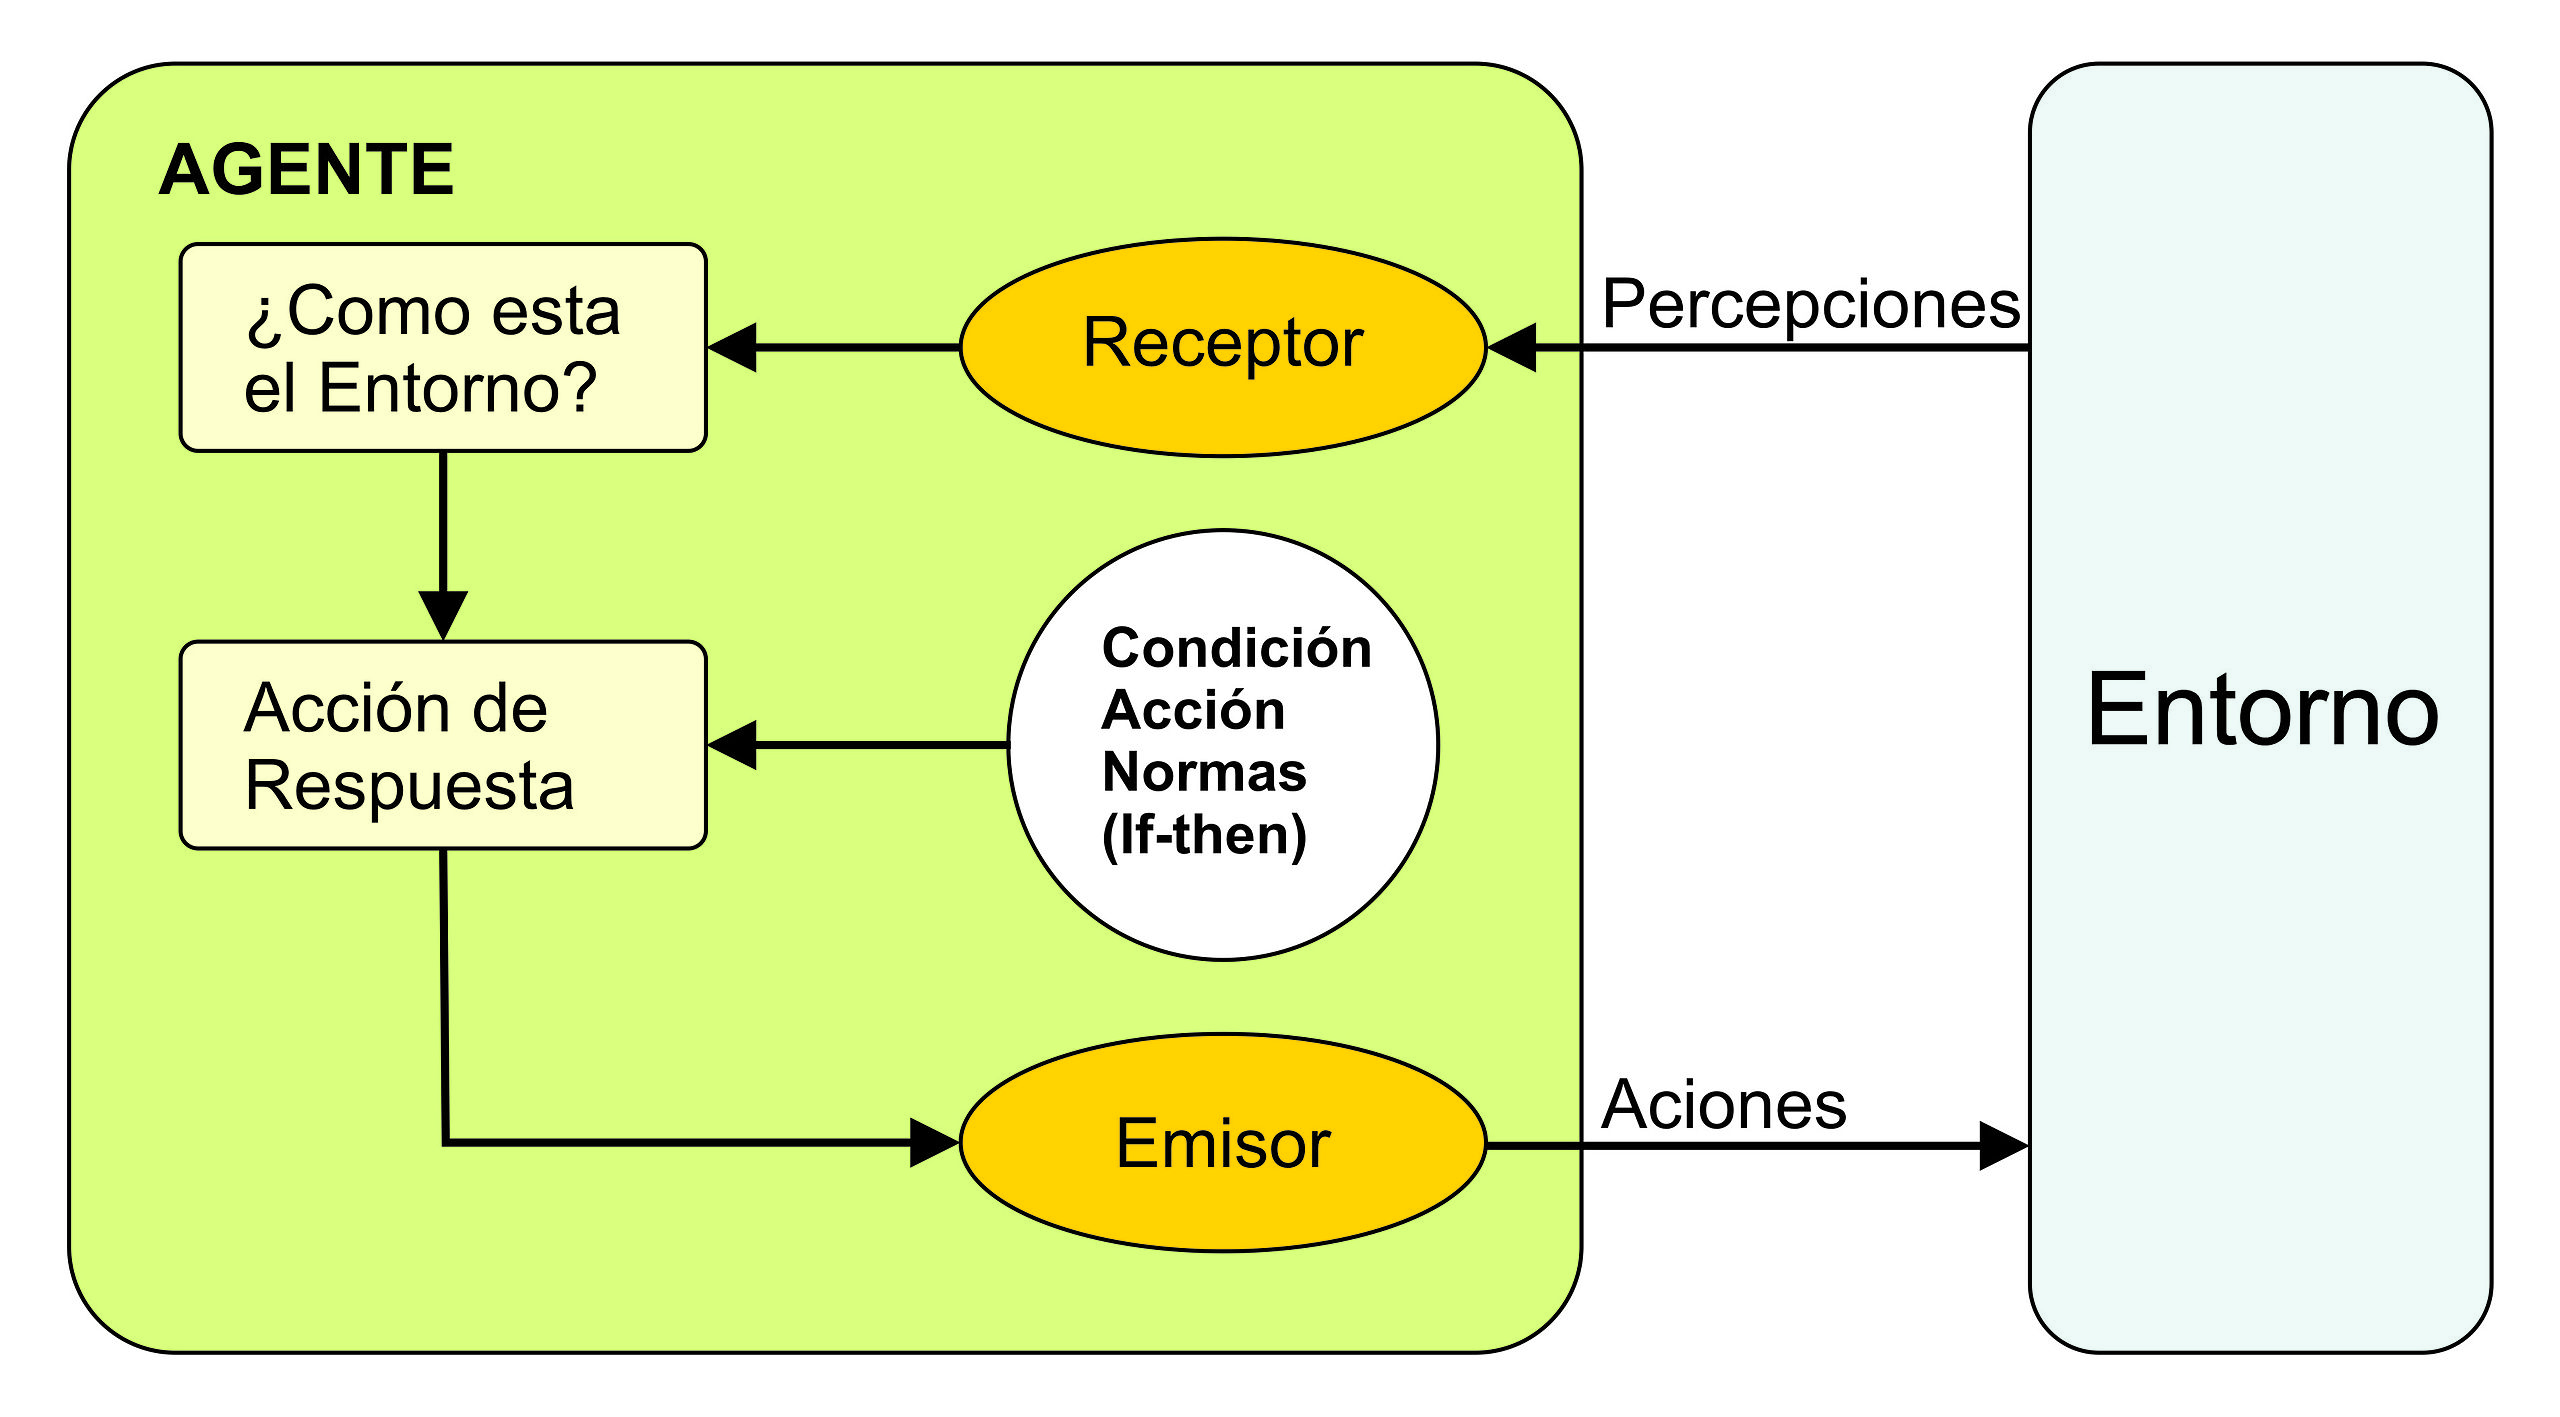
\includegraphics[scale=0.6]{agente}
\caption{Esquema de un agente.}
\end{figure}

Se dice que un agente es inteligente cuando realiza una acci'on sobre su entorno de forma racional,
entendi'endose racional como correcta o beneficiosa. En muchas ocasiones se busca una
maximizaci'on con la obtenci'on del resultado.

Un agente puede ser f'isico o virtual. Posteriormente se presentar'a un ejemplo de agente virtual,
conocido como actor.

Como resumen, podemos decir que un agente debe cumplir las siguiente caracter'isticas:

\begin{itemize}
	\item Percibe el entorno y aprende de 'el.
	\item Se adapta a cambios en su entorno.
	\item Realiza acciones correctas a partir de la informaci'on percibida de su entorno.
	\item Ayuda a alcanzar el objetivo com'un a todos los agentes que componen el sistema.
\end{itemize}

Seg'un su comportamiento, los agentes se pueden clasificar en 6 tipos diferentes \cite{kind-of-agents}, estos son:

\begin{itemize}
	\item Agentes reactivos.
	\item Agentes reactivos basados en modelo.
	\item Agentes basados en objetivos.
	\item Agentes basados en su utilidad.
    \item Agentes que aprenden.
    \item Agentes de consultas.
\end{itemize}

Dado el tipo de arquitecturas que se necesitan hoy d'ia para cumplir una serie de criterios que garanticen
que los sistemas son altamente concurrentes, el tipo de agente que nos interesa a partir de aqu'i son los
agentes reactivos.

Dependiendo del dise'no del sistema, que se describe en el siguiente cap'itulo, los actores a utilizar son
los de tipo reactivo. Pueden incluso estar basados en modelo. Se necesita que el agente, en nuestro caso, y como se ver'a
posteriormente, sea un actor reactivo porque debe responder a cambios. Generalmente, no se necesitan actores que deban
conseguir cumplir objetivos propios.

Tambi'en cabe destacar que los actores tendr'an un comportamiento a menudo social, entendido como que un actor t'ipicamente
necesitar'a de otro para completar una tarea.

Pero antes de entrar en detalle con el modelo de actores, as'i como, el estudio de la capadidad racional de los mismos,
se presenta la capacidad racional en agentes cl'asicos.

\subsection{Capacidad racional en agentes}
\label{sub:capacidad racional en agentes}
El objetivo es conseguir un agente que razone adecuadamente seg'un el medio en el que se encuentre y conseguir dos cosas:

\begin{itemize}
	\item Poder medir en qu'e grado logra ser racional.
	\item Cumplir con el Principio de Racionalidad Restringida de Herbert Simon.
\end{itemize}

En el primer punto, las medidas de rendimiento de un agente pueden variar seg'un el agente, e incluso, no saber que hacer,
enga'narse a s'i mismo, etc. Deben ser adecuadas para cada tipo de agente y al entorno en el que va a actuar.

El segundo punto, se debe conocer en qu'e consiste la racionalidad, y en este caso la misma depende de 4 factores:

\begin{itemize}
	\item Medir el rendimiento que define el 'exito.
	\item Conocimiento del medio en el que se encuentra el agente.
	\item Acciones que el agente puede ejecutar.
	\item Secuencia de percepciones del agente.
\end{itemize}

Un agente, por tanto, tiene que maximizar su rendimiento, para actuar de manera correcta, teniendo en cuenta las
percepciones recibidas hasta ese momento.

\section{Modelo de Actores}
\label{sec:modelos de actores}
En la construcci'on de sistemas de informaci'on se plantea un nuevo mundo, en el cual
las aplicaciones tengan una alta capacidad de respuesta, es decir, que estas sean altamente concurrentes.
Esto se debe a que se necesita mantener la atenci'on y el inter'es de los usuarios que acceden a ellos.

Las diferencias entre estos dos mundos, el mundo que conocemos hasta ahora y el que se plantea
desde hace unos pocos a'nos, cuenta con las siguientes diferencias \cite{RA-HughMcKee}:

\begin{itemize}
	\item Una 'unica computadora frente a un cluster de computadores.
	\item Un 'unico n'ucleo de procesamiento frente a m'ultiples de ellos.
	\item Alto coste de las memorias RAM frente a memorias RAM de bajo coste.
	\item Alto coste del almacenamiento f'isico frente a bajo coste del mismo.
    \item Redes lentas frente a redes de comunicaciones ultra r'apidas.
    \item Baja concurrencia de usuarios frente a alta concurrencia.
    \item Conjunto peque'no de datos frente a grandes conjuntos de datos.
    \item Latencia en segundos frente a latencia en milisegundos.
\end{itemize}

Este modelo, el modelo de actores, fue creado en 1973 por Carl Hewitt y consiste en un modelo
matem'atico de computaci'on concurrente cuya primitiva universal es el actor. En este caso, un actor es
una proci'on de c'odigo software que puede ejecutarse m'ultiples veces, e incluso,
de forma paralela.

Esta idea puede ser llevada m'as all'a gracias a una implementaci'on adecuada de un toolkit
que permita construir sistemas distribuidos siguiendo un modelo de actores y que a su vez
sea fiel al manifiesto reactivo \cite{reactive-manifest}. Pero, no s'olo es una mejora, si no que se hace necesario dado
el entorno en el que se desarrolla y se pretende ejecutar, un computador.

Seguir el manifiesto reactivo ayuda a optimizar los recursos, lo que unido al modelo de actores
resulta en una combinaci'on necesaria para cumplir con el objetivo de concurrencia y alta capacidad
de respuesta.

Existen muchos toolkits o frameworks que implementan este modelo o la mayor parte de 'el. Uno de uso
muy extendido es Akka, construido sobre la JVM y que permite ser utilizado tanto en Java como en Scala.
Una muy buena combinaci'on se obtiene utilizando programaci'on funcional, la cual tiene numerosas
ventajas frente a paradigmas como orientado a objeto, pero que no se comentan aqu'i al no estar
dentro del objetivo de este documento.

\subsection{Qu'e es un actor}
\label{sub:que es un actor}
Un actor, como se ha comentado previamente,  es la primitiva universal de concurrencia
dentro del modelo de actores. Esto es, un bloque de c'odigo por el que pasa un hilo de
ejecuci'on siempre y cuando tenga un mensaje pendiente.

Su topolog'ia consta de un buz'on o cola de mensajes, y el propio actor (c'odigo). Existe un dispatcher
que es el responsable de dar paso a un actor con la entrega de un mensaje del buz'on.
En ese caso, el actor ejecuta la acci'on para la que est'a programado. Una vez finaliza su
ejecuci'on, y dependiendo de la operativa, devolver'a una respuesta, o realizar'a otras acciones,
tales como reenviar el mensaje, crear otro actor para delegar en 'el, etc.

\begin{figure}[h]
\centering
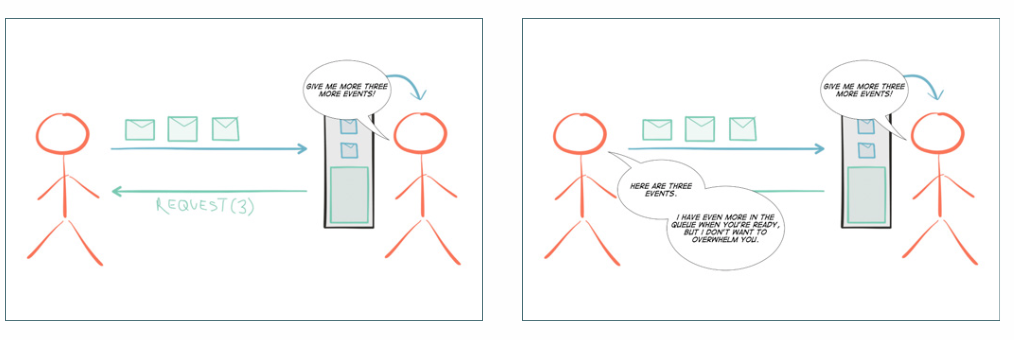
\includegraphics[scale=0.3]{backpressure}
\caption{Comunicaci'on entre agentes mediante t'ecnica de \textit{back-pressure}.}
\end{figure}

Un actor no debe guardar estados, ya que  varios hilos de ejecuci'on pasar'an por el actor,
y en caso de que llegue un mensaje que dependa de un mensaje anterior, el actor podr'ia haber procesado
 otros mensajes previamente que han podido dejar el estado de forma que no permita alcanzar el resultado
 esperado, teniendo por tanto un efecto no deseado.

Es f'acilmente distribuir actores, ya que al ser un paradigma orientado a mensajer'ia, no es
importante el contexto de ejecuci'on, todo su contexto viene dado por el propio mensaje. Existe en
muchos frameworks o toolkits que implementan un modelo de actores la figura del enrutador, que es
la parte del toolkits que permite alojar los actores en m'aquinas remotas facilitando el balanceo de
carga y facilitando tambi'en el aumento de la capacidad de un sistema de forma din'amica.

\subsection{Sistemas distribuidos}
\label{sub:sistemas distribuidos}
Un sistema distribuido se define como un conjunto de computadores conectados entre s'i. Esto
es la soluci'on para poder construir sistemas reactivos.

En un primer momento, los procesadores, construidos con la conocida como tecnolog'a del
silicio, iban doblando su potencia cada 18 meses. Esto es lo que se conoce como Ley de Moore.
Por ello, y gracias tambi'en al avaratamiento de la tecnolog'ia y al aumento de la capacidad de
almacenamiento f'isico y de memoria RAM, no era necesario una alternativa a la construci'on de sistemas
monol'iticos, es decir, sistemas desplegados en un 'unico computador y que contara con
todos los servicios.

Tampoco la sociedad utilizaba internet y los sistemas web para tantas tareas como ahora, por lo
que con un 'unico sistema monol'itico y un computador con suficiente recursos (potencia y memoria)
era suficiente.

A lo largo de los a'nos se ha ido alcanzando los l'imites de la tecnolog'ia y nuevos paradigmas o
enfoques han ido surgiendo. Por ejemplo, casi simult'aneamente a los sistemas distribuidos se
hizo necesario duplicar el numero de procesadores. Es decir, contar con varios n'ucleos de
procesamiento en un mismo procesador.

Los sistemas distribuidos, por tanto, suponen llevar m'as all'a el enfoque aplicado con el enfoque
multin'ucleo, y aplicarlo tambi'en a nivel de computadores aprovechando las redes de comunicaciones
existentes entre ellos.

\subsection{Manifiesto Reactivo}
\label{sub:manifiesto reactivo}
El manifiesto reactivo es un documento en el que se recoge los principios que debe
tener en cuenta todo sistema que pretenda ser reactivo. Esto es, ser flexible, con bajo
acoplamiento y escalables.

Estos principios son los siguientes:

\begin{itemize}
	\item Responsividad: Los sistemas responden de forma adecuada. Se requiere de tiempos
    de respuesta r'apidos y consistentes.
	\item Resilencia: Los sistemas permanecen responsivos incluso en situaci'on de fallo.
    Entendiendo esto como alta disponibilidad. Esto ocurre gracias a la replicaci'on, contenci'on,
    aislamiento y la delegaci'on.
	\item Elasticidad: Los sistemas permanecen responsivos incluso ante variaciones de alta
    carga de trabajo.
	\item Orientaci'on a mensajes: Los sistemas reactivos intercambian mensaje. No mantienen estados,
    si no que el estado es el mensaje. Puede verse como un sistema orientado a eventos u 'ordenes.
\end{itemize}

En este tipo de paradigma, aplicar el manifiesto reactivo se hace necesario, ya que presenta
numerosas ventajas, como por ejemplo, mejor aprovechamiento de los recursos.

\begin{figure}[h]
\centering
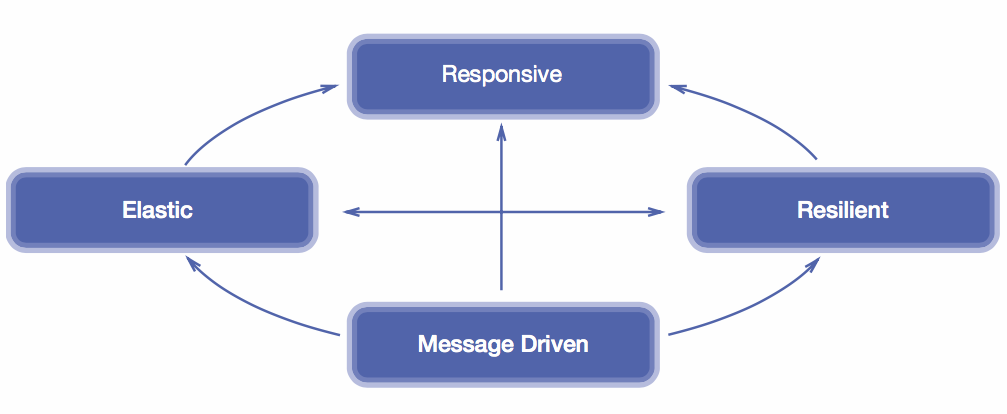
\includegraphics[scale=0.3]{reactivo}
\caption{Relaci'on entre los cuatro principios reactivos.}
\end{figure}

Por tanto, decir que se quiere construir un sistema siguiendo el modelo de actores, es equivalente
a decir que se pretende constuir un sistema reactivo y distribuido.

\subsection{Rol de los actores en sistemas distribuidos (y reactivos)}
\label{sub:rol de los actores en sistemas distribuidos y reactivos}
Quiz'as, en este punto a'un no quede del todo claro por qu'e utilizar actores en sistemas distribuidos.
Es cierto que, un sistema distribuido puede o no estar implementado utilizando actores, pero
si que es de ayuda utilizarlos como manera de simplificar esta tarea.

Los actores permiten que el sistema una vez ha procesado y actuado ante un mensaje o evento, quede
libre para hacer cualquier otra cosa. Esa es en esencia la mayor ventaja que proporciona usar actores.
Pero también facilitan mucho la tarea a la hora de mantener integridad y consistencia en los datos.

\begin{figure}[h]
\centering
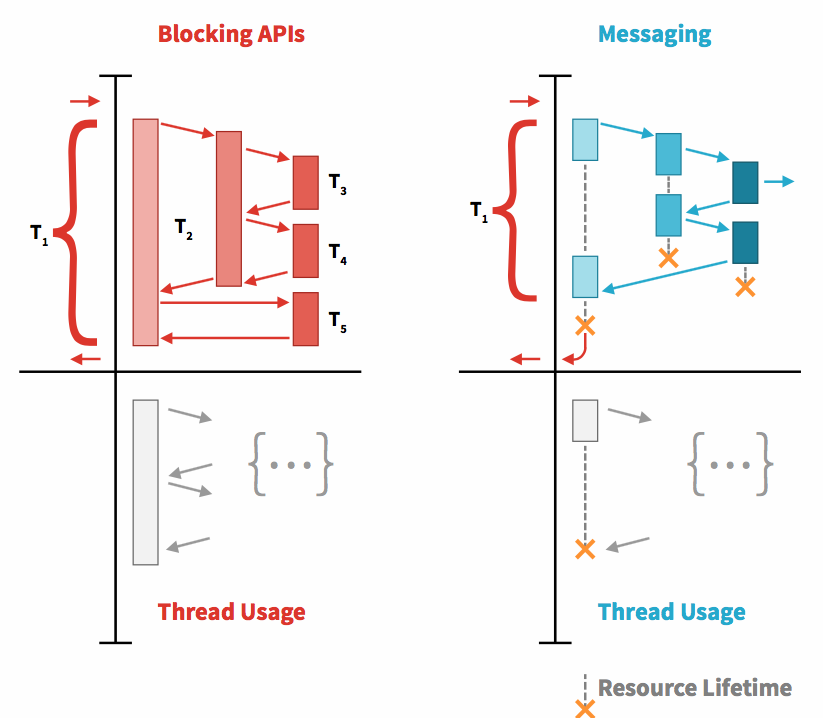
\includegraphics[scale=0.3]{syncvsasync}
\caption{Ejemplo de uso de hilos eficientes en sistemas orientados a mensajer'ia frente a sistemas tradicionales.}
\end{figure}

Sin entrar en detalles, con actores se permite supervisar a otros actores de forma que se pueden
aplicar patrones como Sagas, que ayudan a que el sistema ante un fallo no deje el estado de los datos
de una forma inconsistente.

O, por ejemplo, se puede usar para establecer un patr'on de fallo r'apido, conocido como
Circuit Break, que ayuda a no saturar servicios ante la detecci'on de un problema de respuesta
en el mismo.

\subsection{Capacidad racional en actores}
\label{sub:capacidad racional en actores}
Existen muchos tipos de actores, clasificados seg'un su operativa. Existen actores cuya misi'on
es simplemente hacer de enrutador y/o balanceador. Existen otros cuya misi'on es hacer de conector y
encerrar as'i la l'ogica de comunicaci'on con determinados servicios que usan protocolos espec'ificos.

No se va a catalogar a esos actores como racionales, ya que aunque se obtiene de ellos una respuesta
adecuada en cada momento, no aporta especial valor ya que eso mismo se podr'ia hacer con otros sistemas
que no son considerados como modelo de agente o de actores.

Sin embargo, los actores pueden utilizarse, por ejemplo, para implementar los servicios que permiten
a una entidad financiera hacer transferencias entre clientes. En este caso, se dan dos operaciones desde
un punto de vista muy b'asico, que son:

\begin{itemize}
	\item Retirar el importe del cliente que realiza la transferencia previa comprobaci'on
    de que cuenta con el saldo suficiente.
	\item Agregar dicho importe en el cliente que recibe la transferencia.
\end{itemize}

En un sistema que implemente dichos requisitos, y desarrollado con actores, deben existir los siguientes
actores que se encarguen de realizar la tarea de permitir que se hagan las transferencias sin
que se pierda dinero en el proceso. Tarea que por otro lado no es simple.

Se necesitan, por ejemplo, de acotres que deleguen en otros tareas m'as at'omicas y se encarguen de
supervisar que todos han ido correctamente. Tipicamente, estas tareas se desarrollan en paralelo, y si
una tarea B que est'a asociada a otra tarea A falla, pero la tarea A no, hay que compensar la tarea A.

Otro caso m'as complejo, se da en aquellas entidades que cuentan con un sistema legado que cuenta
con l'ogica en la propia base de datos. Este caso tiene la dificultad de que ante un fallo en el patr'on
que se acaba de describir provoca que un procedimiento de alerta en la base de datos salte
inmediatamente, incluso aunque los actores se encarguen del problema intenando compensar.

En este caso, se puede realizar implementaciones m'as complejas que consisten en grupos de actores
permanentemente activos y divididos en regiones, de manera que se mantiene a cada actor vivo
todo el tiempo para evitar que este tipo de problemas ocurra.

En todos estos casos, los actores ejecutan tareas complejas y dan la respuesta adecuada, es decir, la
respuesta racional en todos los casos, los de 'exitos, y tambi'en los de fallo.

\section{Ventajas e Inconvenientes en el uso de actores}
\label{sec:ventajas e inconvenientes}
Todas las ventajas del uso de actores han sido descritas a lo largo de este documento. Se enumeran las
m'as importantes aqu'i:

\begin{itemize}
	\item Uso eficiente de los recursos en los servidores.
    \item Facilidad de replicaci'on de componentes, servidores y actores.
    \item Mayor capacidad y versatilidad de evoluci'on de una plataforma al ser intercambiables los m'odulos.
    \item Capacidad de soportar m'as concurrencia, e incluso, ser el'astico ante cambios.
\end{itemize}

Pero, tambi'en se presentan inconvenientes en su utilizaci'on:

\begin{itemize}
    \item Necesidad de paradigma funcional en el desarrollo de los actores para ser m'as testable.
    \item Imposibilidad de garant'ia de transacci'on y necesidad de nuevas t'ecnicas para garantizar la integridad de los datos.
    \item Mayor interoperabilidad e integraci'on.
\end{itemize}

\section{Conclusi'on}
Este nuevo paradigma est'a siendo cada vez m'as usado en la industria tecnol'ogica, o incluso, en aquellas industrias
que no tienen origen tecnol'ogico pero que se ven obligados a pivotar hacia dicho sector. Ofrece una soluci'on al mayor
problema de hoy d'ia en los sistemas expuestos en Internet, dar servicio a cada vez m'as usuarios.

En parte, no se ha hecho m'as que reutilizar t'ecnicas o paradigmas utilizados en otros 'areas o industrias. Como en este caso,
que se presentan similitudes entre un modelo de agentes y un modelo de actores.

En el futuro, este parece ser una de las pocas salidas donde poder avanzar y con una alta probabilidad evolucionar a'un m'as
perfeccionando modelos y t'ecnicas ampliamente conocidas. Incluso, extendiendo su uso a sectores o campos en los que no se hace
a'un uso de agentes o actores.

% bibliography
\printbibliography

\end{document}
